
\subsubsection{01.11.14}

\begin{enumerate}
	\item The time of beginning and ending of the congregation:
	16:00 – 21:40
	\item Purposes of the congregation:
	\begin{enumerate}
	  \item Fix rib, that was broken on the last lesson.
	  
	  \item	Set up two axes on the lift.
	  
	  \item	Fix the belt on the lift.
	  
	  \item	Test the lift.
	  
    \end{enumerate}
    
	\item Results:
	\begin{enumerate}
	  \item	It was decided to fix the rip with bolts, becauce it is more fixedly, than hotmelt. In this regard, it had to consolidate above the rest of the ribs to the cap screws do not interfere with the movement of the lift.
      
      \item Two other rips were fixed in holes and fixed with hot melt.
      
      \begin{figure}[H]
      	\begin{minipage}[h]{1\linewidth}
      		\center{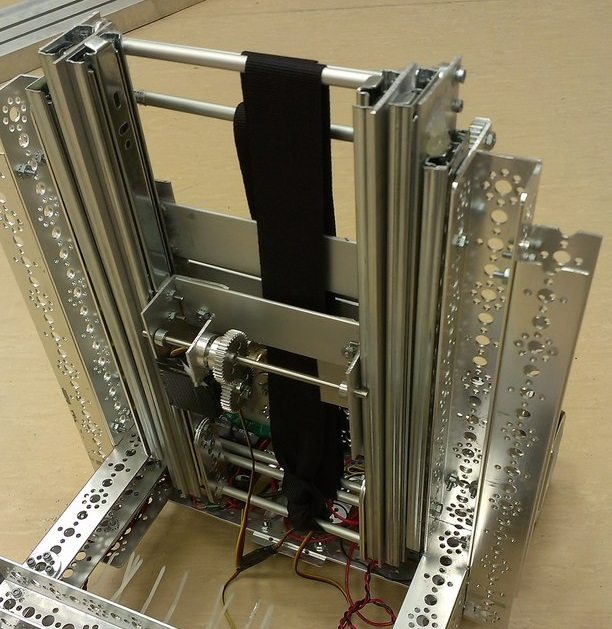
\includegraphics[scale=0.3]{days/01.11.14/images/01}}
      		\caption{Lift is finished}
      	\end{minipage}
      \end{figure}
      
      \item	In testing of lift by pulling the belt by hands, it was found that apart of the lift demands some efforts, which 2 drives must cope. Inner pair rails did not fall under their own weight. it was decided to add weight on it and reduce friction. however, we were not able to do it, becauce we have not detail, tha we need.
      
      \item	On the robot were installed drives for moving of the lift (further mechanism of moving lift will be called "winch").
      
      \begin{figure}[H]
      	\begin{minipage}[h]{1\linewidth}
      		\center{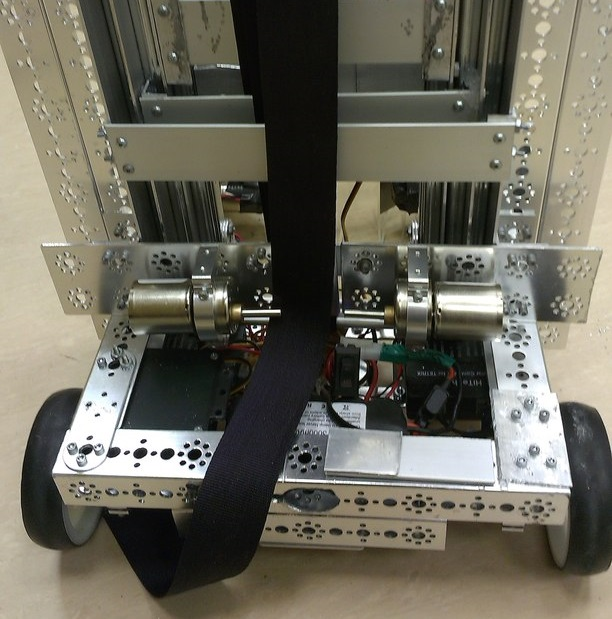
\includegraphics[scale=0.3]{days/01.11.14/images/02}}
      		\caption{Drives for moving lift}
      	\end{minipage}
      \end{figure}
      
    \end{enumerate}
    
	\item Results: 
	\begin{enumerate}
	  \item	The rip was installed.
	  
	  \item	Winch was done.
	  
	  \item	The lift was tested
	  
	  \item	Installation of the winch mechanism was started.
	   
    \end{enumerate}
    
	\item Tasks for the next congregations:
	\begin{enumerate}
	  \item	Finalize the mechanism winch.
	  
	  \item	Install the drivers for the winch.
	  
	  \item	Fix the belt with thread.
	  
	  \item	Replce NXT-brick.
	  
    \end{enumerate}     
\end{enumerate}
\fillpage
